\subsection{Motion History}
\begin{table}[h!]
    \centering
    \begin{tabular}{ | l | c | c | c |}
        \hline
        Konfiguration & Beste & Unter 44 kB & Unter 28 kB \\\hline
        Ensemble-Methode & ExtraTrees & ExtraTrees & ExtraTrees \\\hline
        Maximalhöhe & 10 & 11 & 9 \\\hline
        Waldgröße & 16 & 7 & 6 \\\hline
        Blattgröße (min\_samples\_leaf) & 1 & 2 & 1 \\\hline
        Programmgröße in Bytes & 84200 & 40456 & 22804 \\\hline
        Genauigkeit Testmenge von Klisch & 68,8\% & 67,7\% & 62,5\% \\\hline
        Genauigkeit Gestentestmenge & 74,5\% & 67,6\% & 68,5\% \\\hline
        Genauigkeit Nullgestentestmenge & 68,3\% & 64,4\% & 67,6\% \\\hline
    \end{tabular}
    \caption{Die besten Konfigurationen der Motion History.}
    \label{tab:motion_history}
\end{table}
\begin{figure}[h!]
    \centering
    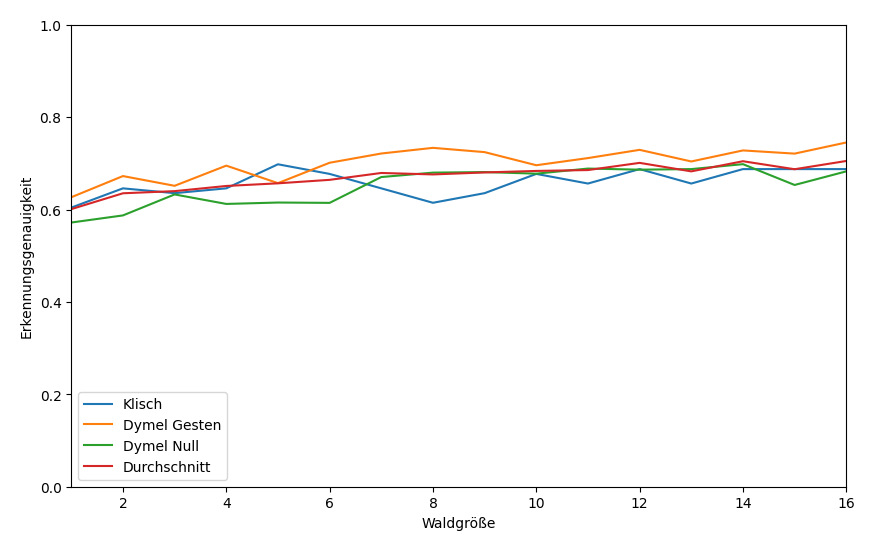
\includegraphics[width=\linewidth]{images/motion_history_acc_per_size.png}
    \caption{Die besten Konfigurationen pro Waldgröße mit Motion History.}
    \label{fig:motion_history_per_forest_size}
\end{figure}
Die Feature-Menge von Motion History beinhaltet für jeden Pixel einen Eintrag, die der Definition des Motion History Image folgen (Formel \ref{formular:mhi}), wobei $\tau=100$ und $\delta=\frac{\tau}{\#Bilder}$ ist.
\newline
\newline
Aus der Tabelle \ref{tab:helligkeitsverteilung} sind die besten Konfigurationen jeder Kategorie zu entnehmen. Die beste Konfiguration wurde mit der Ensemble-Methode \textit{ExtraTrees} gefunden.
Sie erzielt eine Klassifizierungsgenauigkeit von 68,8\% auf der Testmenge von Klisch, 74\% auf der Gestentestmenge und 69\% auf der Nullgestentestmenge. Im Vergleich zu der Helligkeitsverteilung
wird mehr Programmspeicher benötigt und die Gesamtklassifizierungsgenauigkeit ist 1,84\% geringer.
\newline
\newline
Wird die Kategorie \textit{Beste} mit der Kategorie \textit{Unter 28 kB} verglichen, nimmt die Gesamtklassifizierungsgenauigkeit nur um 4,3\% ab. Dabei reduziert sich die Programmgröße um 72,9\%.
Abbildung \ref{fig:motion_history_per_forest_size} zeigt, dass die Klassifizierungsgenauigkeit im Durchschnitt sich mit zunehmender Waldgröße erhöht. Im Vergleich zur Helligkeitsverteilung, ist der Zuwachs größer.
Wenn der Suchraum nicht auf eine Waldgröße von 16 Bäumen begrenzt wäre, würde die beste Konfiguration vermutlich besser sein. Allerdings würde sich auch die Programmgröße signifikant erhöhen.
\newline
\newline
Die Motion History kann mit ausschließlich 8-Bit Integer implementiert werden und hat damit die geringste WCET und Programmgröße pro Baum, weswegen die beste Konfiguration mit einer Waldgröße von 16 Bäumen nicht deutlich
größer ist, als die der Helligkeitsverteilung mit einer Waldgröße von 10 Bäumen.
